\begin{frame}{Transport af Skydevåben (§ 11)}

\vspace{1em}

\begin{columns}[c] % c = center vertically

\column{0.05\textwidth} % Venstre margin

\column{0.7\textwidth} % Midten: Bullets

\small

\raggedright

\begin{itemize}

\itemsep0.6em % Justér afstand mellem bullets

\item \textbf{Formål:} Transport må kun ske i forbindelse med anerkendelsesværdige formål (f.eks. til/fra \structure{opbevaring, anvendelsessted, køb/salg eller reparation}).

\item \textbf{Forsvarlighed:} Våben skal transporteres \textbf{forsvarligt} (f.eks. under konstant tilsyn eller tildækket i aflåst transportmiddel).

\item \textbf{Indpakning:} Skydevåben skal være \structure{indpakket i lukket etui eller lignende} (f.eks. våbenkuffert).

\item \textbf{Ammunition:} Skydevåben må \textbf{IKKE indeholde ammunition} under transport uden for anvendelsesområdet (jagt/skydebane).

\item \textbf{Bæring:} Våben må \textbf{IKKE} transporteres i side- eller skulderhylstre på kroppen.

\end{itemize}

\column{0.25\textwidth} % Højre: Ikon

\centering

\vspace{0pt}

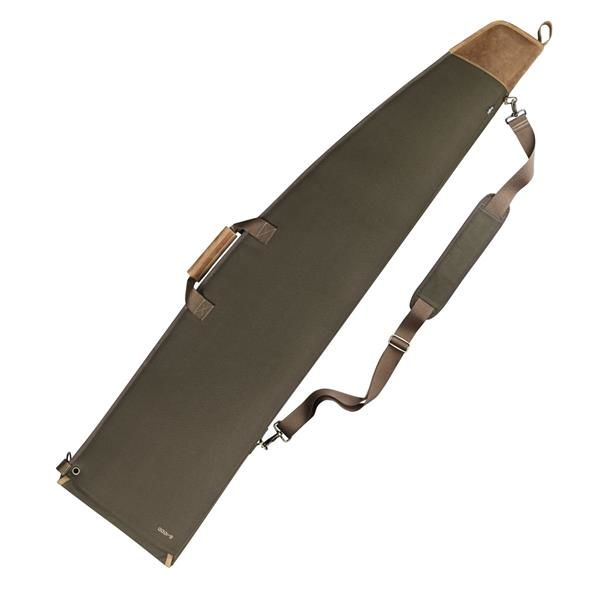
\includegraphics[width=0.9\linewidth]{Billeder/Redskaber/futeral.jpg} % Forslag til et ikon, der symboliserer transport/bil

\end{columns}

\end{frame}